\section{Data Rate}
\label{sec:DataRate}
As ns-3 is a open source simulation software and was used by other researchers in the past too, I used ns-3
to evaluate effect of physical layer configuration on the achievable goodput between two nodes using IEEE 802.11ax Wi-Fi Netdevices
to exchange UDP packets in Adhoc Mode.

The setup consists of two nodes placed in static positions with a distance of \SI{20}{\metre}.
I chose the short communication range setup with no simulated interference to enable wi-Fi transmission without any packets lost.

Every node is equipped with a IEEE 802.11ax Wi-Fi NetDevice which is configured with the default parameters in
\autoref{tab:SimulationDataRate}.
\begin{table}[H]
	\centering
	\begin{tabular}{p{6cm}p{4cm}}
		General Parameters & \\
		\midrule
		Wi-Fi Standard & IEEE 802.11ax\\
		\ac{GI} & \SI{3200}{\nano\second}\\
		Frequency Spectrum & \SI{5.6}{\giga\hertz}\\
		\ac{BW} & \SI{20}{\mega\hertz}\\
		max. Transmission Power & \SI{25}{\decibel}\\
		Antenna Gain & \SI{5}{\dB}\\
		Spatial Streams & 2\\
		\bottomrule
	\end{tabular}
	\caption{Default simulation parameters for Wi-Fi Devices in the goodput simulations}
	\label{tab:SimulationDataRate}
\end{table}

A Constant Rate Wi-Fi Manager is used to set a constant data rate according to the fixed HE-\ac{MCS} for data, non-uniform and control data transmissions.
The used frequency band is \SI{2.4}{\giga\hertz} or \SI{5}{\giga\hertz} as higher frequencies are less resistant to shadowing and fading and a higher data rate is not needed for the \ac{WIC} use cases.
The Wi-Fi Netdevices operate in the frequency channels specified in \autoref{tab:fieldChannels}, which can be used for
outdoor Wi-Fi communication in Germany \cite{freq_plan_24G}, \cite{freq_plan_5G}.

As the Wi-Fi standard implements ACKs for every packet, every lost packet is repeated until it is received or the number of retries is
exceeded.
Platooning Services are time critical and therefore the number of retries should be as low as possible.
This is why additional retransmission mechanisms like TCP are not needed.
Therefore, the chosen transport layer protocol is UDP.

One nodes operate a UDP server and the other one a UDP client.
The client sends \SI{1000}{\byte} UDP packets to the server every \SI{0.1}{\micro\second}.
This packet interval
ensures that the packet queue of the client is never empty after starting the simulation.
The server receives the packets and sends an ACK back to the client.

The simulation runs five times for \SI{5}{\second} for every physical layer configuration.
The goodput for every simulation run is calculated by dividing the number of received bytes at the UDP Server by the simulation time.
The goodput is then averaged over all simulation runs per physical layer configuration and the confidence interval with a confidence level of
\SI{95}{\percent} is calculated.

The theoretical data rate for the different physical layer configurations is retrieved from the function ns3::WifiMode::GetDataRate().

In order to verify the simulation software, I used different methods.
First, I verified,that the theoretical data rate for the IEEE 802.11 ax physical layer configurations in
the simulation is equal to the theoretical data rate specified in the IEEE 802.11ax standard \cite{noauthor_ieee_2021}.

Additionally, I used the MonitorSnifferRxCallback and the MonitorSnifferTxCallback of the ns-3 WifiPhy class to check the ongoing transmissions.
Both Callback functions can be added to WifiPhy objects of Wi-FiNetDevice and are called every time a packet is received or transmitted at the Wi-Fi Netdevice respectively.
The function parameters are Information about the packet, channel frequency and station ID and an instance of the WifiTxVector class. The WifiTxVector instance in the current ns-3 version 3.37 describes all parameters of the transmission inacordance to the TXVECTOR field of the IEEE 802.11 standard \cite{noauthor_ieee_2021}. Additionally, the function parameters of the MonitorSnifferRxCallback contain the signal strength and
the noise power of the received packet.

Using the provided information from the MonitorSnifferRxCallback and the MonitorSnifferTxCallback I was able to comprehend the ongoing transmissions and
verify the simulation results.


\subsubsection*{\acf{GI}}

In the first simulation I varied the \ac{GI} of the Wi-Fi Netdevices for different HE-\ac{MCS} values.
The results are shown in \autoref{fig:Data_rate_GI}. The achieved goodput is plotted against the theoretical data rate for the different \ac{GI} values.
The theoretical data rate is always higher than the achieved goodput of the UDP applications, because the channel is used for \ac{ACK} and ad-hoc Beacon transmissions as well. Due to
these additional transmissions the goodput is lower than the theoretical data rate.
\begin{figure}[H]
	\centering
	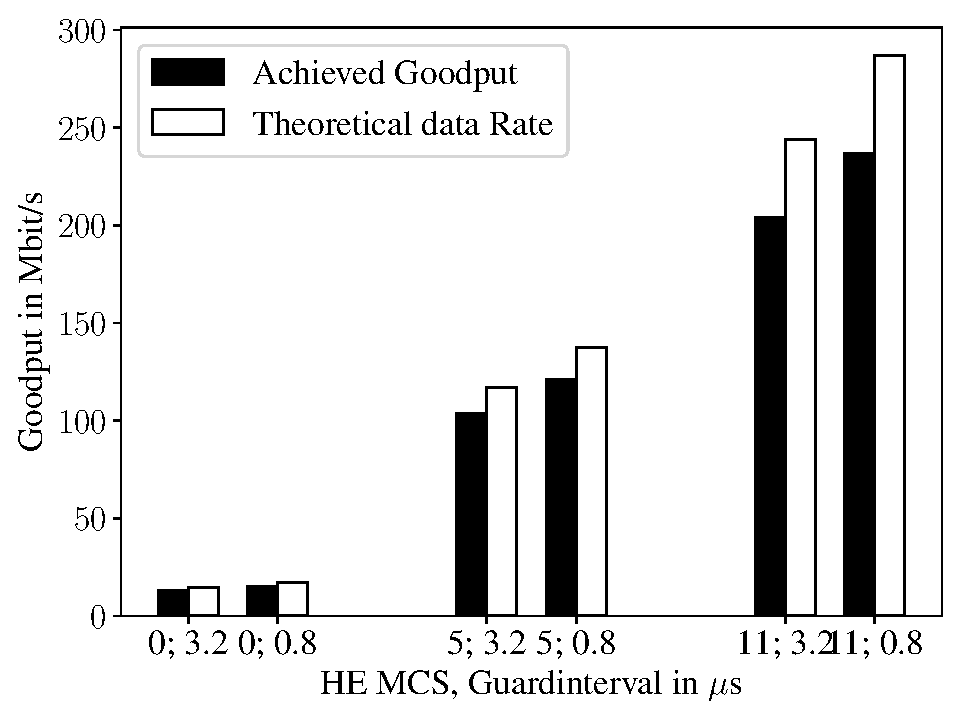
\includegraphics[width=0.95\textwidth]{figures/gi_dataRate_simulation.pdf}
	\caption{Achieved Goodput and theoretical Datarate of two Wi-Fi6 stations in Ad-Hoc Mode with \num{2} \acf{MIMO} streams and a bandwidth of \SI{80}{\mega\hertz} in regards to the number of \acf{MIMO} streams and the chosen HE-\acf{MCS} value}%
	\label{fig:Data_rate_GI}%
\end{figure}

As the \ac{GI} length increases the achieved goodput deceases. This effect can be characterized by the aforementioned formula.
The bandwidth attenuation for the possible \ac{GI} lengths is displayed in \autoref{tab:GIbandwidthAttenuation}.
The effect of the bandwidth attenuation for the different \ac{GI} lengths can be observed in the mean achieved goodput in
\autoref{tab:GIbandwidthAttenuation}, where the decrease of the mean goodput reflects the bandwidth attenuation of the decreasing \ac{GI} length.

A similar effect can be observed whit higher HE-\ac{MCS} values.
\begin{table}[H]
	\centering
	\begin{tabular}{>{\centering}p{3cm}p{3cm}p{3cm}}
		\toprule
		\ac{GI} & Mean achieved goodput & \ac{BW} attentuation\\
		\midrule
		\SI{800}{\nano\second} & \SI{31.15}{\giga\bit\per\second}&
		\SI{94}{\percent} \\
		\SI{1600}{\nano\second} &
		\SI{29.47}{\giga\bit\per\second}&
		\SI{89}{\percent} \\
		\SI{3200}{\nano\second} & \SI{26.52}{\giga\bit\per\second}&
		\SI{80}{\percent} \\
		\bottomrule
	\end{tabular}
	\caption{\acf{BW} attenuation and mean goodput for HE-\ac{MCS}0 in regards to \acf{GI} length}
	\label{tab:GIbandwidthAttenuation}
\end{table}

\textcite{patil_ieee_2020} and \textcite{karmakar_s2-gi_2020} conducted similar simulations
for the \SI{400}{\nano\second} and \SI{800}{\nano\second} \ac{GI} lengths in IEEE 802.11n and IEEE 802.11ac, respectively.
Both papers, state that shorter \ac{GI} lengths lead to higher goodput values under the condition, that there is a short delay spread and a low
channel loss due to interference.

\subsubsection*{\acf{ER} Mode}

In the next simulation I analyzed the effect of the \ac{ER} Mode on the goodput of the IEEE 802.11ax physical layer.
As mentioned in ns-3 Version 3.37, the \ac{ER} Mode is implemented as an \ac{HE} Capability with the new extended WifiPreamble.
But the new Preamble in the \ac{HE} \ac{ER} SU \ac{PPDU} format is not used in ns-3 version3.37.

As I was using the ConstantRateWifiManager, all parameter  for the data transmission are set in the function
ConstantRateWifiManager::DoGetDataTxVector().
The function creates a WifiTxVector instance with the parameters of the
transmission.
There I overwrote the preamble type to the already implemented ns3 WifiPreamble::WIFI\_PREAMBLE\_HE\_ER\_SU, when
the \ac{ER} Mode is enabled and conditions for the \ac{ER} Mode in the IEEE 802.11ax standard \cite{noauthor_ieee_2021} are fulfilled.
Ns-3 version 3.37 implements ns3::GlobalValue, which allow users to set global values for the simulation, which can be accessed
in every class without changing Constructor or function parameters.
This leaves the original functionality of the ns3 code intact.

I used the ns3::GlobalValue to create an instance named HE\_ER\_Mode, which is set to true at the start and read in the ns3::ConstantRateWifiManager::DoGetDataTxVector() function
to overwrite the preamble type.

Via the MonitorSnifferRxCallback and the MonitorSnifferTxCallback I was able to verify, that the ns3 WifiPreamble::WIFI\_PREAMBLE\_HE\_ER\_SU was used
for data transmission, when the following conditions were met: a) the \ac{ER} Mode is enabled, b) the number of spatial streams is \num{1}, c) the HE-\ac{MCS} value is less than \num{3} and
d) the \ac{BW} is \SI{20}{\mega\hertz}.

The results of the simulation are shown in \autoref{fig:Data_rate_ER}, where the lost achieved goodput is plotted against the theoretical data rate for the different HE-\ac{MCS} values.
The lost goodput is calculated by subtracting the achieved goodput when using the normal \ac{HE} \ac{ER} mode from the achieved goodput when using the \ac{HE} SU mode.
The only difference between \ac{HE} SU and \ac{HE} \ac{ER} SU transmissions is the preamble, which repeats the HE-SIG-A field in the \ac{HE} \ac{ER} SU \ac{PPDU} format.
This results in a longer transmission time, which reflects in the lower achieved goodput for the \ac{ER} Mode.
\begin{figure}[H]%
	\centering
	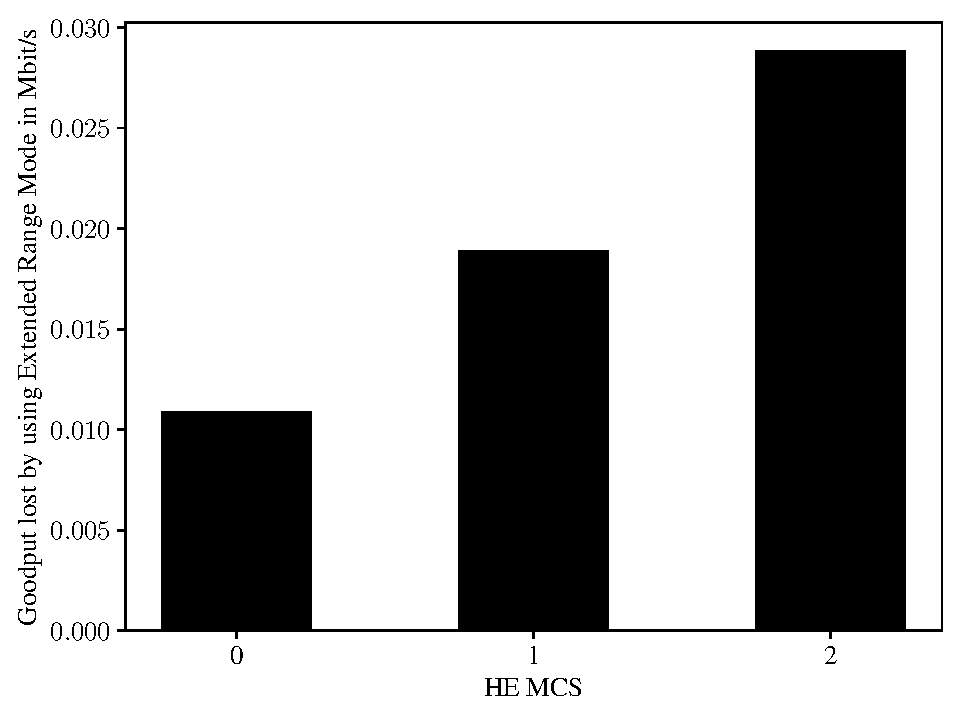
\includegraphics[width=0.95\textwidth]{figures/ER_dataRate_simulation.pdf}
	\caption{Achieved Goodput and theoretical Datarate of two Wi-Fi6 stations in Ad-Hoc Mode with a \acf{GI} of \SI{3200}{\nano\second} and a bandwidth of \SI{20}{\mega\hertz} in regards to the number of \acf{MIMO} streams and the chosen HE-\ac{MCS} value}%
	\label{fig:Data_rate_ER}%
\end{figure}
The effect increases with smaller packet sizes, because the longer transmission time of preamble is more significant for smaller packets.
For higher HE-\ac{MCS} values more achievable goodput is lost, because longer transmission time for the preamble could have
been used more \ac{OFDM} symbol transmissions, where more data is coded onto a symbol.

\subsubsection*{\acf{DCM}}
Using the \ac{DCM} in the IEEE 802.11ax physical layer has also an effect on the achievable goodput.
As aforementioned, the \ac{DCM} is not supported by ns-3 version 3.37.
Therefore, I implemented the \ac{DCM} for this simulation in the ns-3 version 3.37 by transmitting a payload of twice the size, which represents the original payload and a
copy of the original payload for the HE-\ac{MCS} values 0, 1, 3 and 4, where \ac{MCS} is allowed.
Using \ac{DCM}, the receiver would apply maximum likelihood decoding to decode the original payload with a higher probability.

The results of the simulation are shown in \autoref{fig:Data_rate_DCM}, where the lost achieved goodput is plotted against
the theoretical data rate for the different HE-\ac{MCS} values.
The theoretical data rate while using \ac{DCM} is half of the
theoretical data rate without \ac{DCM}, which complies with the IEEE 802.11ax standard \cite{noauthor_ieee_2021}.
\begin{figure}[H]%
	\centering
	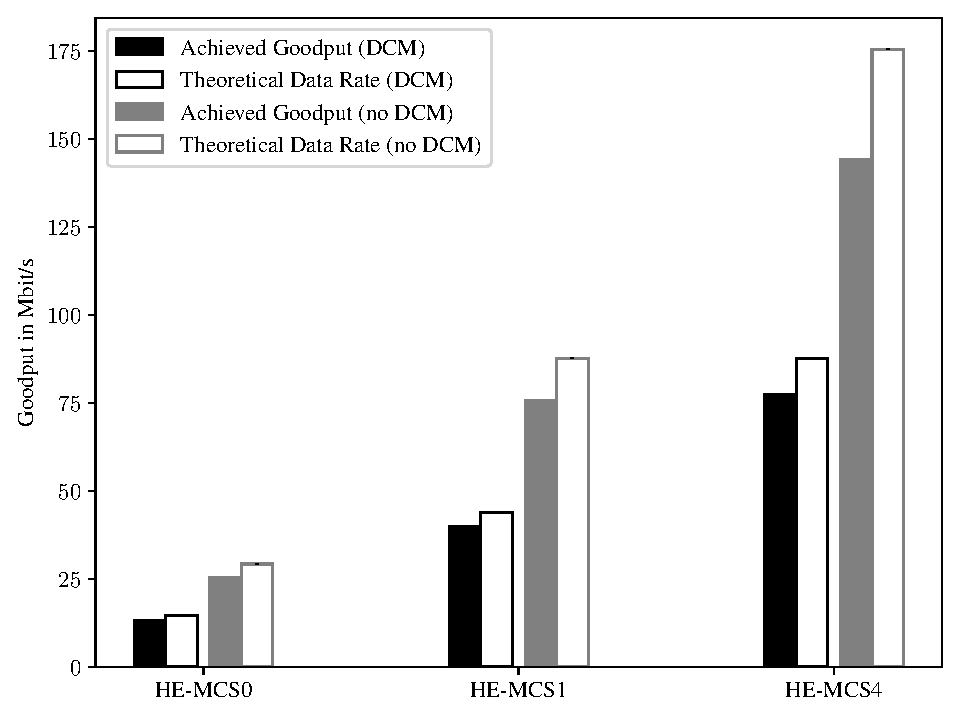
\includegraphics[width=0.95\textwidth]{figures/DCM_dataRate_simulation.pdf}
	\caption{Achieved Goodput and theoretical Datarate of two Wi-Fi6 stations in Ad-Hoc Mode with for IEEE 802.11ax physical layer parameters of a \acf{GI} of \SI{3200}{\nano\second}, a \acf{BW} of \SI{20}{\mega\hertz} and 2 spatial streams  in regards to the number of the chosen HE-\acf{MCS} value and whether \acf{DCM} is enabled}%
	\label{fig:Data_rate_DCM}%
\end{figure}

The achieved goodput is always lower than the theoretical data rate, because data transmission time is lost to the header overhead and media access time.
WiFi access is based on CSMA CA, which means that the stations have to wait for a random time before they can transmit on a free channel.
Additionally, the channel can be occupied by ACK or adhoc beacon frames, which also have to be transmitted.

Using \ac{DCM} increases the ratio of achievable goodput to theoretical data rate, because only one header and one ACK frame is transmitted per
\SI{2000}{\byte} payload and the node has to go to the medium access procedure only once per \SI{2000}{\byte} payload.


\begin{comment}
	sommer
	header_fixed  medium access (beacon, ACK, RTS, CTS) the achievable goodput is always lower than the theoretical data rate.
	theoretical data rate
\end{comment}




\subsubsection*{\acf{STBC}}
Another physical layer parameter, which reduces the theoretical data rate for more robustness is the \ac{STBC}.
As mentioned, ns-3 version 3.37 does not support the \ac{STBC} for the IEEE 802.11ax standard.
Therefore, I reduced the number of
\ac{MIMO} streams from two to one, when the \ac{STBC} is enabled. \ac{STBC} would transmit a redundant copy of the data on the second antenna, which would be combined
using the space-time block code (STBC) to increase the robustness and reliability of the transmission.
The results of the simulation are shown in \autoref{fig:Data_rate_STBC}, where the lost achieved goodput is plotted against
the theoretical data rate for the different HE-\ac{MCS} values.
The theoretical data rate while using \ac{STBC} is half of the theoretical data rate without \ac{STBC},
which complies with the IEEE 802.11ax standard \cite{noauthor_ieee_2021}.
\begin{figure}[H]%
	\centering
	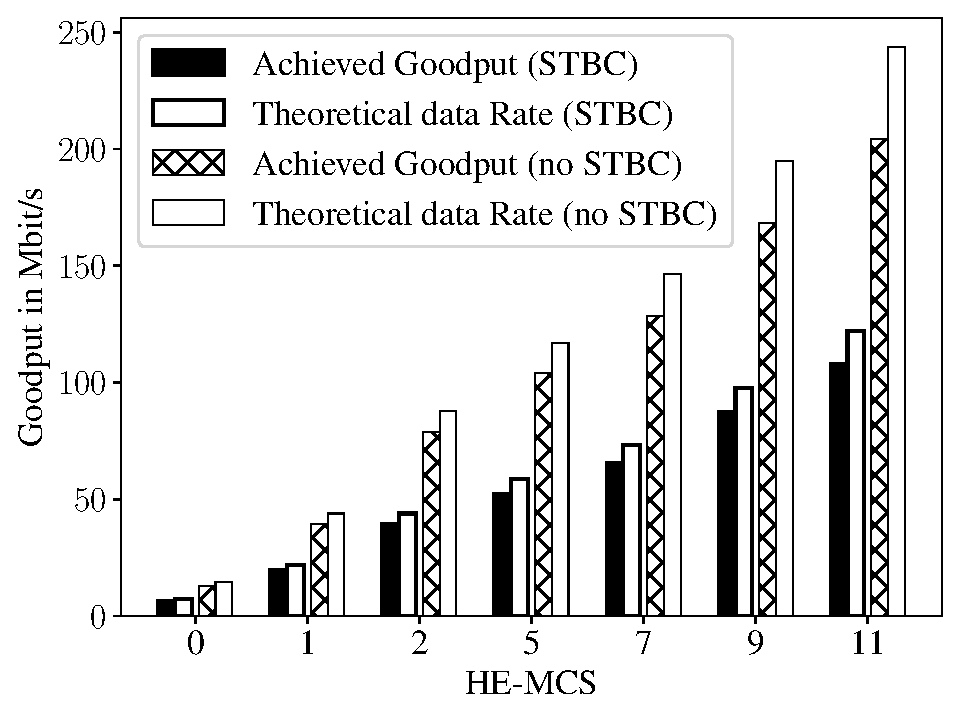
\includegraphics[width=0.95\textwidth]{figures/STBC_dataRate_simulation}
	\caption{Achieved Goodput and theoretical Datarate of two WiFi 6 stations in Ad-Hoc Mode with for IEEE 802.11ax physical layer parameters of a \acf{GI} of \SI{3200}{\nano\second}, a \acf{BW} of \SI{20}{\mega\hertz} and 2 spatial streams  in regards to the number of the chosen HE-\acf{MCS} value and whether \acf{STBC} is enabled}%
	\label{fig:Data_rate_STBC}%
\end{figure}

Other physical layer parameters, which are supported by the IEEE 802.11ax standard are \ac{LDPC} and utilizing more \ac{MIMO} streams.
The effect, that using more \ac{MIMO} streams for a transmission increases the achievable goodput
is already known \cite{sauter_wireless_2022, noauthor_ieee_2021, noauthor_ieee_2021-1}.
\ac{LDPC} no new effect for data rate, but more robustness which results in a lower \ac{PER}.

\todo[color=yellow]{2.4 GHZ?}


\begin{figure}[H]%
	\centering
	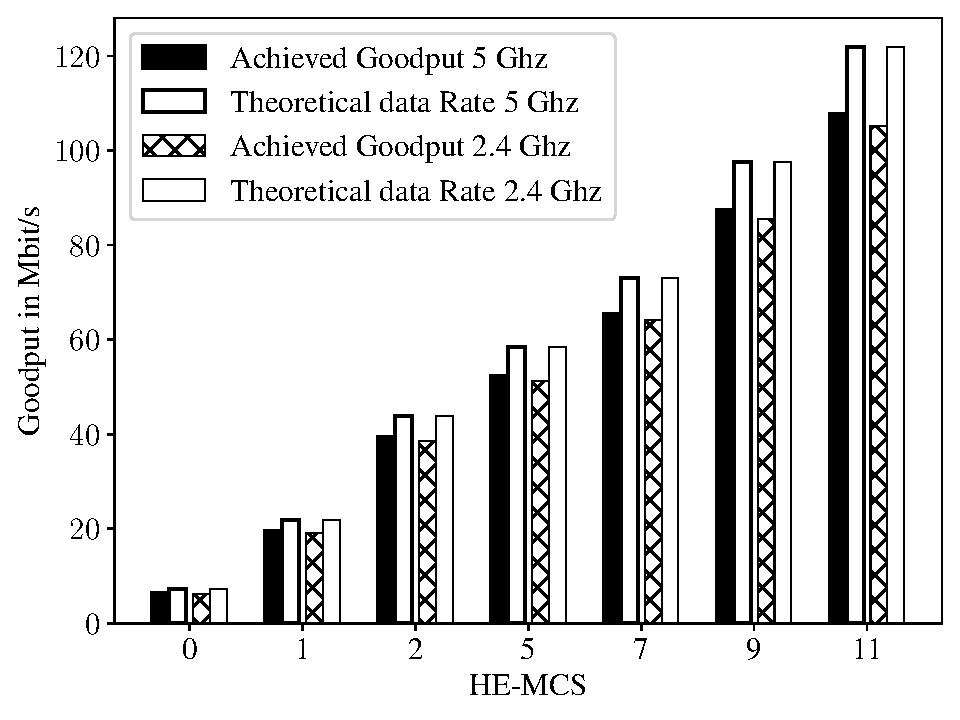
\includegraphics[width=0.95\textwidth]{figures/STBC_dataRate_simulation24}
	\caption{Achieved Goodput and theoretical Datarate of two WiFi 6 stations in Ad-Hoc Mode with for IEEE 802.11ax
		physical layer parameters of a \acf{GI} of \SI{3200}{\nano\second}, a \acf{BW} of \SI{20}{\mega\hertz} and 2 spatial streams,
		\ac{STBC} enabled and in regards to the number of the chosen HE-\acf{MCS} value and whether the
		\SI{2.4}{\giga\hertz} or \SI{5}{\giga\hertz} frequency spectrum is used}%
	\label{fig:Data_rate_STBC24}%
\end{figure}